\section {Power plane}

\begin{figure}[h]
  \centering
  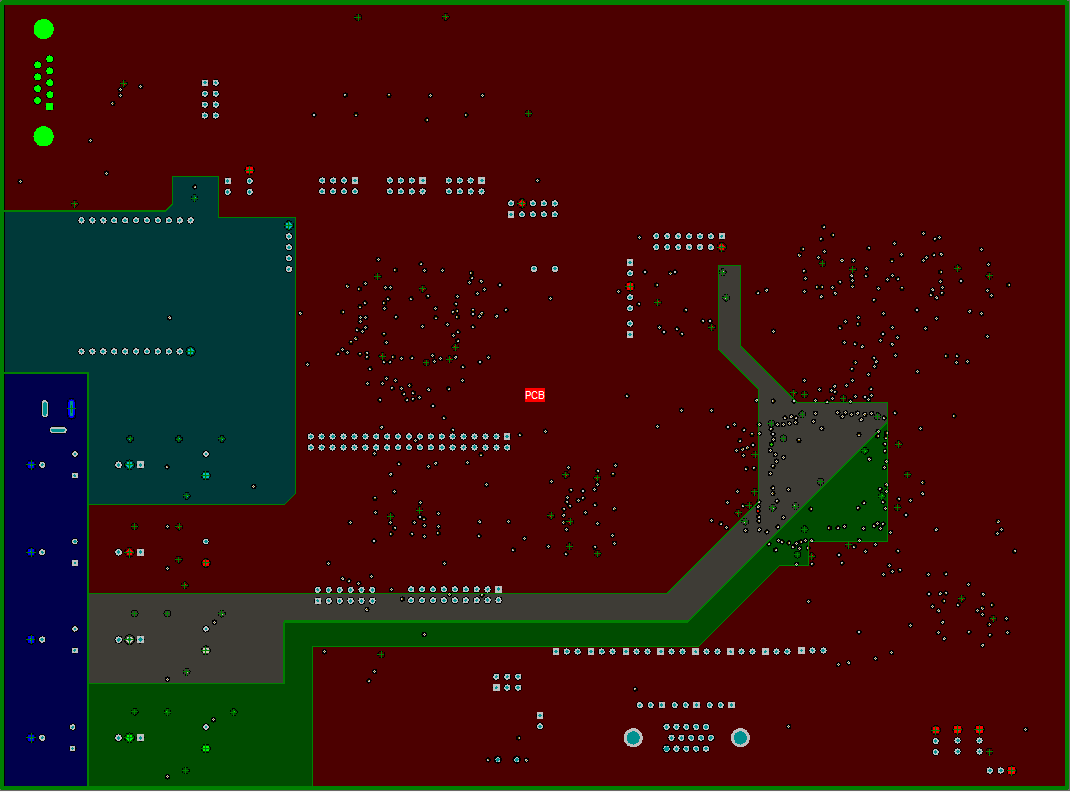
\includegraphics[width=0.8\textwidth]{fig/pcb/power_planes.PNG}
  \caption{The Power Planes}
  \label{fig:power_planes}
\end{figure}


Since our power supply was exactly the same as Festina Lente's we also ended up
with similar power planes, as seen on the figure above; 12V (dark blue), 5V (teal), 
3.3V (red), 2.5V (gray) and 1.2V (green). The 5V was only used for the external 
\ac{VGA} controller. 2.5V and 1.2V were split across the \ac{FPGA}.

The rest of the board got 3.3V. The entire power plane was put in internal layer
1, with a ground layer in internal layer 2.
